\documentclass{article}
\usepackage{civ}
\newcommand*{\tabbox}[2][t]{%
    \vspace{0pt}\parbox[#1][3.7\baselineskip]{1cm}{\strut#2\strut}}
\title{CIV102: Problem Set \#6}
\author{QiLin Xue \\ \href{mailto:qilin.xue@mail.utoronto.ca}{qilin.xue@mail.utoronto.ca} \\ TA: Michel}
\everymath{\displaystyle}
\usepackage{multirow}
\date{\today}
\usepackage{mathrsfs}
\usetikzlibrary{arrows}
\usepackage{siunitx}
\usepackage{wasysym}
\usetikzlibrary{calc}
\usepackage{xcolor}
\setlength\parindent{0pt}
% \setlength\extrarowheight{10pt}
\renewcommand{\arraystretch}{2}
\usepackage{adjustbox}
\begin{document}
\maketitle
\section{Problem One: Bracing for the Bottom}
We can first calculate the load due to the force at each joint by considering the area of the tributary area to be $3 \times 1.2 = 3.6\si{\meter\squared}$ for each joint that is not at the edge for a force of $2\si{\kilo\pascal} \times 3.6 \si{\meter\square} = 7.2\si{\kilo\newton}$. To maintain static equilibrium, the ends of the bridge must exert a force of $\frac{1}{2}7 \cdot 7.2 = 25.2\si{\kilo\newton}$ in the opposite direction. The systems diagram should look like this:
\begin{center}
    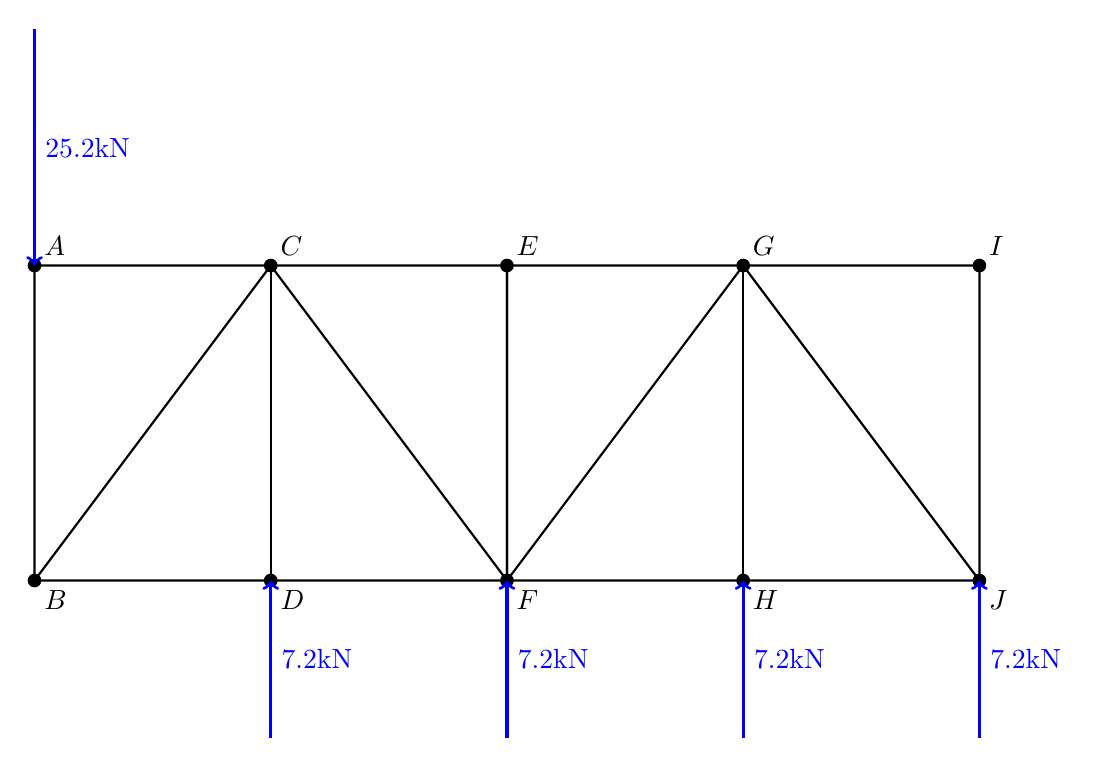
\begin{tikzpicture}
        \coordinate (A) at (0,4);
        \coordinate (B) at (0,0);
        \coordinate (C) at (3,4);
        \coordinate (D) at (3,0);
        \coordinate (E) at (6,4);
        \coordinate (F) at (6,0);
        \coordinate (G) at (9,4);
        \coordinate (H) at (9,0);
        \coordinate (I) at (12,4);
        \coordinate (J) at (12,0);
        % \coordinate (K) at (15,4);
        % \coordinate (L) at (15,0);
        % \coordinate (M) at (18,4);
        % \coordinate (N) at (18,0);
        % \coordinate (O) at (21,4);
        % \coordinate (P) at (21,0);
        % \coordinate (Q) at (24,4);
        % \coordinate (R) at (24,0);

        \draw[fill=black] (A) circle (0.08) node[above right] {$A$};
        \draw[fill=black] (B) circle (0.08) node[below right] {$B$};
        \draw[fill=black] (C) circle (0.08) node[above right] {$C$};
        \draw[fill=black] (D) circle (0.08) node[below right] {$D$};
        \draw[fill=black] (E) circle (0.08) node[above right] {$E$};
        \draw[fill=black] (F) circle (0.08) node[below right] {$F$};
        \draw[fill=black] (G) circle (0.08) node[above right] {$G$};
        \draw[fill=black] (H) circle (0.08) node[below right] {$H$};
        \draw[fill=black] (I) circle (0.08) node[above right] {$I$};
        \draw[fill=black] (J) circle (0.08) node[below right] {$J$};

        \foreach \i in {0,6}{
            \draw[thick] (\i,0) -- (\i,4) -- (\i+3,4) -- (\i+6,4) -- (\i+6,0) -- (\i+3,0) -- (\i,0) -- (\i+3,4) -- (\i+6,0);
            \draw[thick] (\i+3,0) -- (\i+3,4);
        }

        \draw[very thick, blue, <-] (D) -- ++(0,-2) node[midway,right] {$7.2\si{\kilo\newton}$};
        \draw[very thick, blue, <-] (F) -- ++(0,-2) node[midway,right] {$7.2\si{\kilo\newton}$};
        \draw[very thick, blue, <-] (H) -- ++(0,-2) node[midway,right] {$7.2\si{\kilo\newton}$};
        \draw[very thick, blue, <-] (J) -- ++(0,-2) node[midway,right] {$7.2\si{\kilo\newton}$};
        \draw[very thick, blue, <-] (A) -- ++(0,3) node[midway,right] {$25.2\si{\kilo\newton}$};
    \end{tikzpicture}
\end{center}
where we have only drawn one half, due to the symmetry of the bridge. Before we start analyzing joints, note that we can identify the zero force members easily. Whenever three forces act upon a joint, if one of the members is perpendicular to the other two forces, then it will be a zero force member. Therefore, $AC$, $EF$, $GH$, and $IJ$ will all be zero force members.

Since we neglect the horizontal members, we only care about the vertical forces. So balancing forces on $A$, we see that:
\begin{equation}
    \sum F_y = 0 \implies AB+25.2 = 0 \implies AB=-25.2\si{\kilo\newton} 
    \label{eq:}
\end{equation}
and balancing forces on $D$ and $H$, we see that all of their vertical members have a force (compression) equal to:
\begin{equation}
    CD = GH = -7.2\si{\kilo\newton}.
    \label{eq:}
\end{equation}
Balancing forces on $B$, we have:
\begin{equation}
    \sum F_y = 0 \implies AB+BC_y=0 \implies BC_y = -AB = 25.2\si{\kilo\newton}
    \label{eq:}
\end{equation}
Note that I calculated the vertical component of $BC$, denoted as $BC_y$. This is purely a stylistic choice that makes the intermediate calculations simpler. Balancing forces on $C$, we have:
\begin{equation}
    \sum F_y= 0 \implies BC_y+CD+CF_y=0 \implies CF_y=-CD-BC_y=-18\si{\kilo\newton}
    \label{eq:}
\end{equation}
Balancing forces on $F$, we have:
\begin{equation}
    \sum F_y = 0 \implies CF_y+FG_y+7.2=0\implies FG_y=-CF_y-7.2=10.8\si{\kilo\newton}
    \label{eq:}
\end{equation}
and balancing forces on $G$ gives:
\begin{equation}
    \sum F_y = 0\implies FG_y+GH+GJ_y = 0 \implies GJ_y=-GH-FG_y=-3.6\si{\kilo\newton}
    \label{eq:}
\end{equation}
We have all the vertical forces, so to convert these to their actual compression and tension values, we can use the fact that the triangles are a 3-4-5 special triangle, so:
\begin{equation}
    F = \frac{5}{4}F_y
    \label{eq:}
\end{equation}
giving us:
\begin{itemize}
    \item $AB=-25.2\si{\kilo\newton}$
    \item $BC=31.5\si{\kilo\newton}$
    \item $CF=-22.5\si{\kilo\newton}$
    \item $FG=13.5\si{\kilo\newton}$
    \item $GJ=-4.5\si{\kilo\newton}$
\end{itemize}
Note that if the wind came from the opposite side, then the direction of the force in the diagonal braces would switch (and the vertical members would switch from being in compression to being a zero force member, and vice versa).

The reason why this is the case isn't immediately clear. If the wind came from the other direction, then joints $D$ and $H$ would not experience a wind load and as a result $CD$ and $GH$ would be zero force members. We would then start our analysis from joint $B$ to see that $BC$ is in compression instead of tension. All the vertical forces at each joint (which is attached to the diagonal braces) would also switch direction, so the calculations would be the exact same except with a different parity.

As a result, $BC$ will be the largest in compression, which will have the following parameters:
\begin{align}
    A_\text{min} &= 2\frac{F}{\sigma_y} = 180 \si{\milli\meter\squared}\\ 
    I_\text{min} &= 3\frac{FL^2}{\pi^2 E} = 1.197 \times 10^6 \si{\milli\meter\tothe{4}}\\ 
    r_\text{min} &= \frac{L}{200}  = 25.0\si{\milli\meter}
\end{align}
And the lightest HSS that satisfies these conditions is $\boxed{\text{89x89x4.8}}$.

\newpage
\section{Problem Two: Other Loads}
\textbf{(a)} We can draw a diagram (excluding the hand rails) of the elevation view:
\begin{center}
    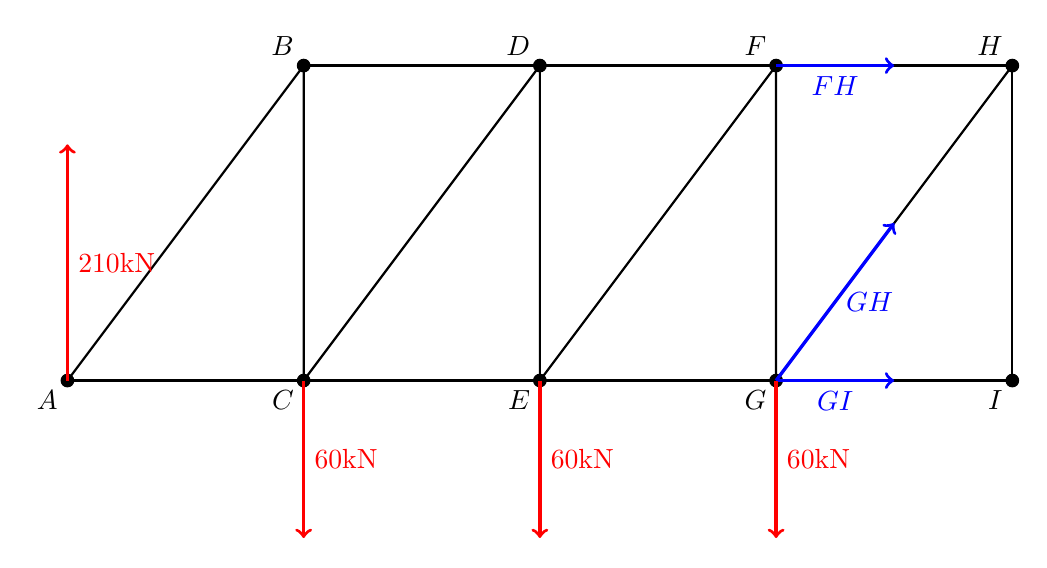
\begin{tikzpicture}
        \coordinate (A) at (0,0);
        \coordinate (B) at (3,4);
        \coordinate (C) at (3,0);
        \coordinate (D) at (6,4);
        \coordinate (E) at (6,0);
        \coordinate (F) at (9,4);
        \coordinate (G) at (9,0);
        \coordinate (H) at (12,4);
        \coordinate (I) at (12,0);

        \draw[fill=black] (A) circle (0.08) node[below left] {$A$};
        \draw[fill=black] (B) circle (0.08) node[above left] {$B$};
        \draw[fill=black] (C) circle (0.08) node[below left] {$C$};
        \draw[fill=black] (D) circle (0.08) node[above left] {$D$};
        \draw[fill=black] (E) circle (0.08) node[below left] {$E$};
        \draw[fill=black] (F) circle (0.08) node[above left] {$F$};
        \draw[fill=black] (G) circle (0.08) node[below left] {$G$};
        \draw[fill=black] (H) circle (0.08) node[above left] {$H$};
        \draw[fill=black] (I) circle (0.08) node[below left] {$I$};

        \draw[thick] (A) -- (C) -- (E) -- (G) -- (I) -- (H) -- (F) -- (D) -- (B);
        \draw[thick] (A) -- (B) -- (C) -- (D) -- (E) -- (F) -- (G) -- (H);
        
        \draw[blue,very thick,->] (F) -- ($(F) !0.5! (H)$) node[midway,below] {$FH$};
        \draw[blue,very thick,->] (G) -- ($(G) !0.5! (H)$) node[midway,right] {$GH$};
        \draw[blue,very thick,->] (G) -- ($(G) !0.5! (I)$) node[midway,below] {$GI$};

        \draw[red,very thick,->] (C) -- ++(0,-2) node[midway, right] {$60\si{\kilo\newton}$};
        \draw[red,very thick,->] (E) -- ++(0,-2) node[midway, right] {$60\si{\kilo\newton}$};
        \draw[red,very thick,->] (G) -- ++(0,-2) node[midway, right] {$60\si{\kilo\newton}$};
        \draw[red,very thick,->] (A) -- ++(0,3) node[midway, right] {$210\si{\kilo\newton}$};

    \end{tikzpicture}
\end{center}
The gravity load exerted at each joint is given by $10\si{\kilo\pascal} \times (3\si{\meter} \cdot 2\si{\meter})=60\si{\kilo\newton}$, so the reaction forces at the ends are equal to:
\begin{equation}
    R = \frac{7\cdot 60}{2} = 210\si{\kilo\newton}
    \label{eq:}
\end{equation}
To determine the compressive force in the top chord and in the web, we can cut through members $FH$, $GH$, and $GI$. We can balance forces and moments to get:
\begin{align}
    \sum F_y = 0 &\implies 210+GH\frac{4}{5}=60\cdot 3 \implies GH=-37.5\si{\kilo\newton}\\ 
    \sum M_\text{about A} = 0 &\implies 60(3)+60(6)+60(9)+FH(4)=GH\frac{4}{5}(9) \implies FH = -337.5\si{\kilo\newton} \\ 
    \sum F_x = 0 &\implies FH+GH\frac{3}{5}+GI=0 \implies GI = 360\si{\kilo\newton}
    \label{eq:}
\end{align}
Balancing forces on joint $A$, we get:
\begin{align}
    \sum F_y = 0 &\implies 210+AB\frac{4}{5}=0\implies AB=-262.5\si{\kilo\newton} \\ 
    \sum F_x = 0 &\implies AB\frac{3}{5}+AC = 0 \implies AC = 157.5\si{\kilo\newton}
    \label{eq:}
\end{align}
The highest member in compression is member $FH=-337.5\si{\kilo\newton}$, but we also need to take into account member $AB=-262.5\si{\kilo\newton}$ since the member is longer, as well as the highest member in tension $GI=360\si{\kilo\newton}.$ Our requirements are:
\begin{align}
    A_\text{min} &= 2\frac{F}{\sigma_y} = 2060 \si{\milli\meter\squared}\\ 
    I_\text{min} &= 3\frac{FL^2}{\pi^2 E} = 9.97 \times 10^6 \si{\milli\meter\tothe{4}}\\ 
    r_\text{min} &= \frac{L}{200}  = 25.0\si{\milli\meter}
\end{align}
which gives us the HSS of $\boxed{\text{178x178x4.8}}$.

\textbf{(b)} To perform wind calculations, we must first find the wind loads. The tributary area for joints $D$ and $E$ is given by:
\begin{equation}
    0.178 \text{ m} \times \left(1.5+1.5+2+2.5\right) = 1.335\si{\meter\squared}.
    \label{eq:}
\end{equation}
for joint $H$ (note that there is an additional diagonal brace):
\begin{equation}
    0.178 \text{ m} \times \left(1.5+1.5+2+2.5+2.5\right) = 1.780\si{\meter\squared}.
    \label{eq:}
\end{equation}
and for joint $B$:
\begin{equation}
    0.178 \text{ m} \times \left(1.5+2+2.5\right) = 1.068\si{\meter\squared}.
    \label{eq:}
\end{equation}
leading to forces of $F=2.67\si{\kilo\newton}$, $F=3.56\si{\kilo\newton}$, and $F=2.136\si{\kilo\newton}$ respectively. The bracing forces are thus:
\begin{equation}
    R = \left(2\cdot 2.67+\frac{1}{2}3.56+2.136\right)=9.256\si{\kilo\newton}
    \label{eq:}
\end{equation}
We can summarize this in a diagram:
\begin{center}
    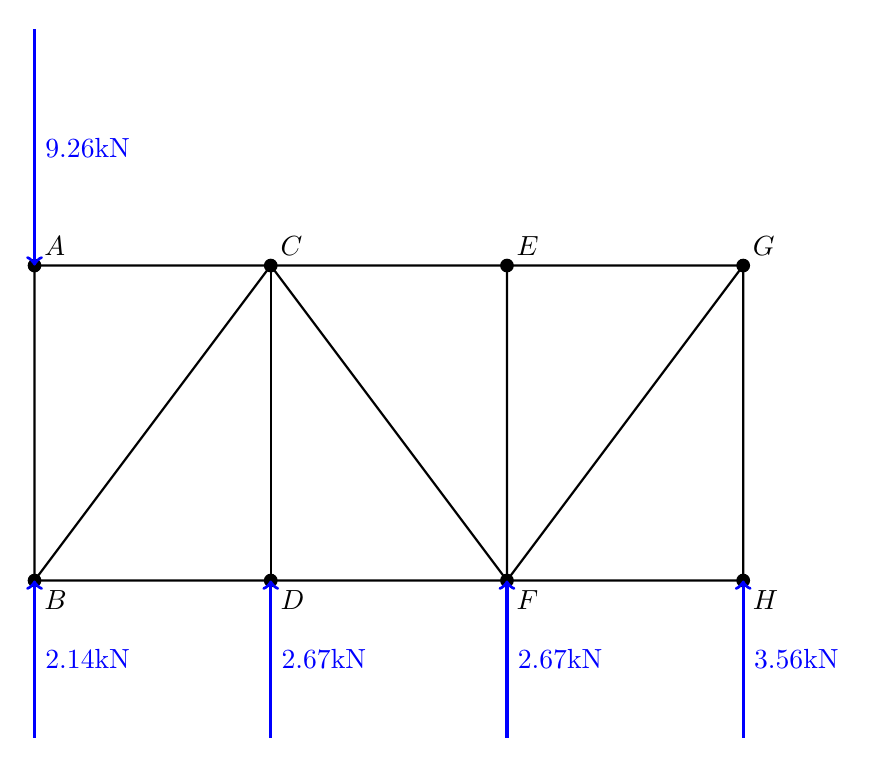
\begin{tikzpicture}
        \coordinate (A) at (0,4);
        \coordinate (B) at (0,0);
        \coordinate (C) at (3,4);
        \coordinate (D) at (3,0);
        \coordinate (E) at (6,4);
        \coordinate (F) at (6,0);
        \coordinate (G) at (9,4);
        \coordinate (H) at (9,0);
        % \coordinate (K) at (15,4);
        % \coordinate (L) at (15,0);
        % \coordinate (M) at (18,4);
        % \coordinate (N) at (18,0);
        % \coordinate (O) at (21,4);
        % \coordinate (P) at (21,0);
        % \coordinate (Q) at (24,4);
        % \coordinate (R) at (24,0);

        \draw[fill=black] (A) circle (0.08) node[above right] {$A$};
        \draw[fill=black] (B) circle (0.08) node[below right] {$B$};
        \draw[fill=black] (C) circle (0.08) node[above right] {$C$};
        \draw[fill=black] (D) circle (0.08) node[below right] {$D$};
        \draw[fill=black] (E) circle (0.08) node[above right] {$E$};
        \draw[fill=black] (F) circle (0.08) node[below right] {$F$};
        \draw[fill=black] (G) circle (0.08) node[above right] {$G$};
        \draw[fill=black] (H) circle (0.08) node[below right] {$H$};

        \draw[thick] (0,0) -- (0,4) -- (3,4) -- (6,4) -- (6,0) -- (3,0) -- (0,0) -- (3,4) -- (6,0);
        \draw[thick] (3,0) -- (3,4);
        \draw[thick] (E) -- (G) -- (H) -- (F) -- (G);
        \draw[very thick, blue, <-] (B) -- ++(0,-2) node[midway,right] {$2.14\si{\kilo\newton}$};

        \draw[very thick, blue, <-] (D) -- ++(0,-2) node[midway,right] {$2.67\si{\kilo\newton}$};
        \draw[very thick, blue, <-] (F) -- ++(0,-2) node[midway,right] {$2.67\si{\kilo\newton}$};
        \draw[very thick, blue, <-] (H) -- ++(0,-2) node[midway,right] {$3.56\si{\kilo\newton}$};
        \draw[very thick, blue, <-] (A) -- ++(0,3) node[midway,right] {$9.26 \si{\kilo\newton}$};
    \end{tikzpicture}
\end{center}
Similar to part (a), $EF$ is a zero force member and the other vertical members have forces of $CD=-2.67\si{\kilo\newton}$ and $GH=-3.56\si{\kilo\newton}$. We can start our joint analysis from $A$, looking at only vertical forces, to get:
\begin{equation}
    \sum F_y = 0 \implies AB+7.12=0 \implies AB=-9.26\si{\kilo\newton}
    \label{eq:}
\end{equation}
For joint $B$:
\begin{equation}
    \sum F_y = 0 \implies AB+BC_y+2.14 = 0 \implies BC_y = 7.12\si{\kilo\newton}
    \label{eq:}
\end{equation}
For joint $C$:
\begin{equation}
    \sum F_y = 0 \implies BC_y+(-2.67)+CF_y = 0 \implies CF_y = 2.67-BC_y=-4.45\si{\kilo\newton}
    \label{eq:}
\end{equation}
For joint $F$:
\begin{equation}
    \sum F_y = 0 \implies CF_y + 2.67 + FG_y =0 \implies FG_y = -2.67-CF_y=1.78\si{\kilo\newton}
    \label{eq:}
\end{equation}
For all diagonal braces, we can multiply their vertical force by $\frac{5}{4}$ to get their actual compression and tension values, which gives us:
\begin{itemize}
    \item $AB=-9.26\si{\kilo\newton}$
    \item $BC=8.90\si{\kilo\newton}$
    \item $CD=-2.67\si{\kilo\newton}$
    \item $CF=-5.56(25)\si{\kilo\newton}$
    \item $FG=2.22(5) \si{\kilo\newton}$
    \item $GH=-3.56\si{\kilo\newton}$
\end{itemize}
Following the same reasoning as before, if the wind load instead came from the opposite side, the diagonal members would switch from being compression and tension and the vertical members switch between loaded and unloaded.

\textbf{(c)} The highest member that could possibly be in compression is $AB=-9.26\si{\kilo\newton}$ and $BC=-8.9\si{\kilo\newton}$, which yields the following constraints:
\begin{align}
    A_\text{min} &= 2\frac{F}{\sigma_y} = 52.9 \si{\milli\meter\squared}\\ 
    I_\text{min} &= 3\frac{FL^2}{\pi^2 E} = 0.338 \times 10^6 \si{\milli\meter\tothe{4}}\\ 
    r_\text{min} &= \frac{L}{200}  = 25.0\si{\milli\meter}
\end{align}
which gives the lightest HSS as $\boxed{\text{76x76x4.8}}$.
\newpage
\section{Problem 3: Stability}
\textbf{(a)} Refer to the diagram drawn in problem two. The top member (in elevation view) with the highest compression forces is $FH=-337.5\si{\kilo\newton}$. In order to maintain lateral stability the brace forces required to restrain it is:
\begin{equation}
    R = 0.02|FH|=6.75\si{\kilo\newton}
    \label{eq:}
\end{equation}
We can draw a diagram of the elevation view, assuming that the only forces are due to the bracing (e.g. ignoring wind). There are two cases to consider, depending on what buckles:

\textbf{Case 1:} Top Buckles:
\begin{center}
    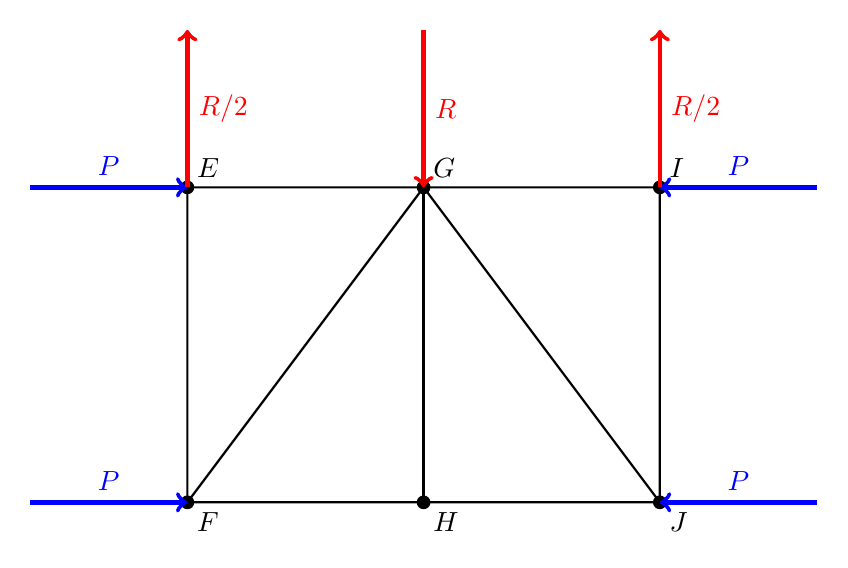
\begin{tikzpicture}
        % \coordinate (A) at (0,4);
        % \coordinate (B) at (0,0);
        % \coordinate (C) at (3,4);
        % \coordinate (D) at (3,0);
        \coordinate (E) at (6,4);
        \coordinate (F) at (6,0);
        \coordinate (G) at (9,4);
        \coordinate (H) at (9,0);
        \coordinate (I) at (12,4);
        \coordinate (J) at (12,0);
        % \coordinate (M) at (18,4);
        % \coordinate (N) at (18,0);
        % \coordinate (O) at (21,4);
        % \coordinate (P) at (21,0);
        % \coordinate (Q) at (24,4);
        % \coordinate (R) at (24,0);

        % \draw[fill=black] (A) circle (0.08) node[above right] {$A$};
        % \draw[fill=black] (B) circle (0.08) node[below right] {$B$};
        % \draw[fill=black] (C) circle (0.08) node[above right] {$C$};
        % \draw[fill=black] (D) circle (0.08) node[below right] {$D$};
        \draw[fill=black] (E) circle (0.08) node[above right] {$E$};
        \draw[fill=black] (F) circle (0.08) node[below right] {$F$};
        \draw[fill=black] (G) circle (0.08) node[above right] {$G$};
        \draw[fill=black] (H) circle (0.08) node[below right] {$H$};
        \draw[fill=black] (I) circle (0.08) node[above right] {$I$};
        \draw[fill=black] (J) circle (0.08) node[below right] {$J$};

        \draw[thick] (F) -- (E) -- (G) -- (I) -- (J) -- (H) -- (F) -- (G) -- (J);
        \draw[thick] (G) -- (H);
        \draw[ultra thick, blue, <-] (E) -- ++(-2,0) node[midway,above] {$P$};
        \draw[ultra thick, blue, <-] (F) -- ++(-2,0) node[midway,above] {$P$};
        \draw[ultra thick, blue, <-] (I) -- ++(2,0) node[midway,above] {$P$};
        \draw[ultra thick, blue, <-] (J) -- ++(2,0) node[midway,above] {$P$};

        \draw[ultra thick, red, <-] (G) -- ++(0,2) node[midway,right] {$R$};
        \draw[ultra thick, red, ->] (E) -- ++(0,2) node[midway,right] {$R/2$};
        \draw[ultra thick, red, ->] (I) -- ++(0,2) node[midway,right] {$R/2$};

        % \draw[very thick, blue, <-] (H) -- ++(0,-2) node[midway,right] {$3.56\si{\kilo\newton}$};
        % \draw[very thick, blue, <-] (A) -- ++(0,3) node[midway,right] {$7.12\si{\kilo\newton}$};
    \end{tikzpicture}
\end{center}
We can identify $GH$ as a zero force member since it is perpendicular to $FH$ and $HJ$ and performing a force balance on the joint $F$ gives the brace force $FG$ as:
\begin{equation}
    FG\frac{4}{5} = R/2 \implies FG=-\frac{5}{4}R/2=-4.21(875)\si{\kilo\newton}
    \label{eq:}
\end{equation}
\textbf{Case 2:} Bottom Buckles:
\begin{center}
    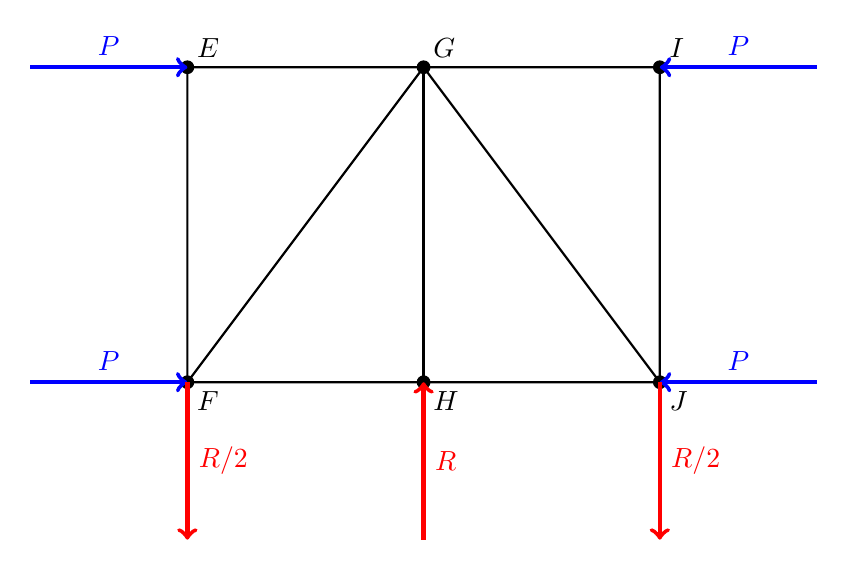
\begin{tikzpicture}
        % \coordinate (A) at (0,4);
        % \coordinate (B) at (0,0);
        % \coordinate (C) at (3,4);
        % \coordinate (D) at (3,0);
        \coordinate (E) at (6,4);
        \coordinate (F) at (6,0);
        \coordinate (G) at (9,4);
        \coordinate (H) at (9,0);
        \coordinate (I) at (12,4);
        \coordinate (J) at (12,0);
        % \coordinate (M) at (18,4);
        % \coordinate (N) at (18,0);
        % \coordinate (O) at (21,4);
        % \coordinate (P) at (21,0);
        % \coordinate (Q) at (24,4);
        % \coordinate (R) at (24,0);

        % \draw[fill=black] (A) circle (0.08) node[above right] {$A$};
        % \draw[fill=black] (B) circle (0.08) node[below right] {$B$};
        % \draw[fill=black] (C) circle (0.08) node[above right] {$C$};
        % \draw[fill=black] (D) circle (0.08) node[below right] {$D$};
        \draw[fill=black] (E) circle (0.08) node[above right] {$E$};
        \draw[fill=black] (F) circle (0.08) node[below right] {$F$};
        \draw[fill=black] (G) circle (0.08) node[above right] {$G$};
        \draw[fill=black] (H) circle (0.08) node[below right] {$H$};
        \draw[fill=black] (I) circle (0.08) node[above right] {$I$};
        \draw[fill=black] (J) circle (0.08) node[below right] {$J$};

        \draw[thick] (F) -- (E) -- (G) -- (I) -- (J) -- (H) -- (F) -- (G) -- (J);
        \draw[thick] (G) -- (H);
        \draw[ultra thick, blue, <-] (E) -- ++(-2,0) node[midway,above] {$P$};
        \draw[ultra thick, blue, <-] (F) -- ++(-2,0) node[midway,above] {$P$};
        \draw[ultra thick, blue, <-] (I) -- ++(2,0) node[midway,above] {$P$};
        \draw[ultra thick, blue, <-] (J) -- ++(2,0) node[midway,above] {$P$};

        \draw[ultra thick, red, <-] (H) -- ++(0,-2) node[midway,right] {$R$};
        \draw[ultra thick, red, ->] (F) -- ++(0,-2) node[midway,right] {$R/2$};
        \draw[ultra thick, red, ->] (J) -- ++(0,-2) node[midway,right] {$R/2$};

        % \draw[very thick, blue, <-] (H) -- ++(0,-2) node[midway,right] {$3.56\si{\kilo\newton}$};
        % \draw[very thick, blue, <-] (A) -- ++(0,3) node[midway,right] {$7.12\si{\kilo\newton}$};
    \end{tikzpicture}
\end{center}
Here, $EF$ will be a zero force member, and $FG$ will take on the same magnitude as before of $\boxed{FG=4.22\si{\kilo\newton}}$, but flipped. The only difference is that $GH$ will no longer be a zero force member and will be equal to the reaction force $\boxed{GH=-6.75\si{\kilo\newton}}.$

\textbf{(b)} The maximum forces in compression are $FG=-4.22\si{\kilo\newton}$ and $GH=-6.75\si{\kilo\newton}$.
\begin{align}
    A_\text{min} &= 2\frac{F}{\sigma_y} = 38.6 \si{\milli\meter\squared}\\ 
    I_\text{min} &= 3\frac{FL^2}{\pi^2 E} = 0.1603 \times 10^6 \si{\milli\meter\tothe{4}}\\ 
    r_\text{min} &= \frac{L}{200}  = 25.0\si{\milli\meter}
\end{align}
so the HSS chosen in question two still holds.

\newpage
\section{Problem 4: Virtual Loads}
We begin by drawing the systems diagarm:
\begin{center}
    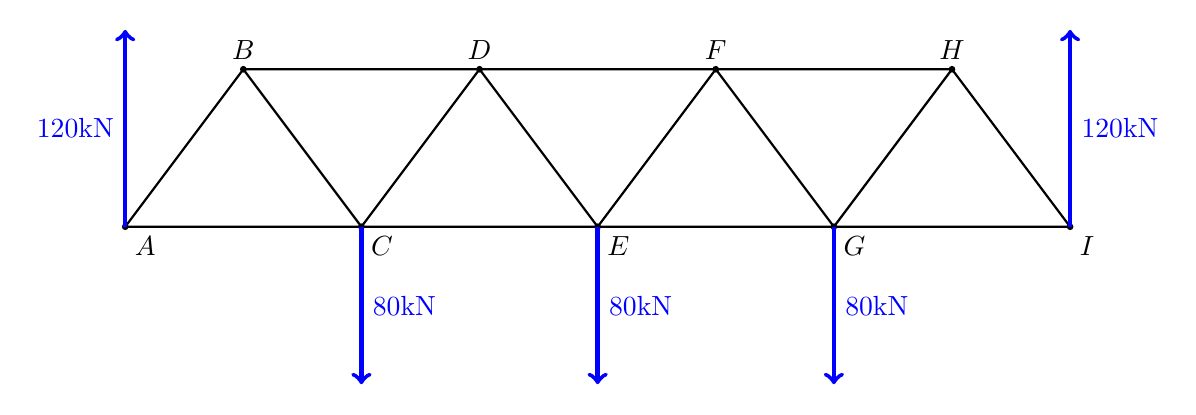
\begin{tikzpicture}[scale=0.5]
        \coordinate (A) at (0,0);
        \coordinate (B) at (3,4);
        \coordinate (C) at (6,0);
        \coordinate (D) at (9,4);
        \coordinate (E) at (12,0);
        \coordinate (F) at (15,4);
        \coordinate (G) at (18,0);
        \coordinate (H) at (21,4);
        \coordinate (I) at (24,0);

        \draw[fill=black] (A) circle (0.07) node[below right] {$A$};
        \draw[fill=black] (C) circle (0.07) node[below right] {$C$};
        \draw[fill=black] (E) circle (0.07) node[below right] {$E$};
        \draw[fill=black] (G) circle (0.07) node[below right] {$G$};
        \draw[fill=black] (I) circle (0.07) node[below right] {$I$};

        \draw[fill=black] (B) circle (0.07) node[above] {$B$};
        \draw[fill=black] (D) circle (0.07) node[above] {$D$};
        \draw[fill=black] (F) circle (0.07) node[above] {$F$};
        \draw[fill=black] (H) circle (0.07) node[above] {$H$};
        
        \draw[thick] (B) -- (D) -- (F) -- (H) -- (I) -- (G) -- (E) -- (C) -- (A) -- (B) -- (C) -- (D) -- (E) -- (F) -- (G) -- (H);

        \draw[ultra thick, color=blue, ->] (C) --++ (0,-4) node[midway,right] {$80\si{\kilo\newton}$};
        \draw[ultra thick, color=blue, ->] (E) --++ (0,-4) node[midway,right] {$80\si{\kilo\newton}$};
        \draw[ultra thick, color=blue, ->] (G) --++ (0,-4) node[midway,right] {$80\si{\kilo\newton}$};

        \draw[ultra thick, color=blue, ->] (A) --++ (0,5) node[midway,left] {$120\si{\kilo\newton}$};
        \draw[ultra thick, color=blue, ->] (I) --++ (0,5) node[midway,right] {$120\si{\kilo\newton}$};
    \end{tikzpicture}
\end{center}
We can begin by looking at the vertical component of the diagonal forces. Only focusing on the left half of the bridge due to symmetry, we get:
\begin{center}
    \begin{tabular}{|c|c|c|}
        \hline
        Vertical Component           & Horizontal Component         & Actual Force                 \\ \hline
        $AB_y=-120\si{\kilo\newton}$ & $AB_x=-90\si{\kilo\newton}$ & $AB=-150\si{\kilo\newton}$ \\ \hline
        $BC_y=120\si{\kilo\newton}$ & $BC_x=90\si{\kilo\newton}$ & $BC=-150\si{\kilo\newton}$ \\ \hline
        $CD_y=-40\si{\kilo\newton}$ & $CD_x=-30\si{\kilo\newton}$ & $CD=-50\si{\kilo\newton}$ \\ \hline
        $DE_y=-40\si{\kilo\newton}$ & $DE_x=30\si{\kilo\newton}$ & $DE=-50\si{\kilo\newton}$ \\ \hline
        \end{tabular}
\end{center}
The first column was determined by looking at only the vertical components at each joint while the second and third columns were determined by multiplying the first column by the ratio $3/4$ and $5/4$, respectively. Using the second column, we can easily figure out the force of each horizontal member:
\begin{align}
    AC&=90\si{\kilo\newton} \\ 
    CE&=210\si{\kilo\newton} \\ 
    BD&=-180\si{\kilo\newton} \\ 
    DF&=-240\si{\kilo\newton}
\end{align}
To determine our virtual forces, we can put a downwards dummy force with magnitude $1\si{\kilo\newton}$ at joint $E$. Then the reaction forces are $0.5\si{\kilo\newton}$, and solving for the forces in the same way, we get:
\begin{center}
    \begin{tabular}{|c|c|c|}
        \hline
        Vertical Component           & Horizontal Component         & Actual Force                 \\ \hline
        $AB_y^*=-0.5\si{\kilo\newton}$ & $AB_x^*=-0.375\si{\kilo\newton}$ & $AB ^*=-0.625\si{\kilo\newton}$ \\ \hline
        $BC_y^*=0.5\si{\kilo\newton}$ & $BC_x ^*=0.375\si{\kilo\newton}$ & $BC  ^*=0.625\si{\kilo\newton}$ \\ \hline
        $CD_y^*=-0.5\si{\kilo\newton}$ & $CD_x^* =-0.375\si{\kilo\newton}$ & $CD^*=-0.625\si{\kilo\newton}$ \\ \hline
        $DE_y^*=0.5\si{\kilo\newton}$ & $DE_x ^*=0.375\si{\kilo\newton}$ & $DE  ^*=-0.625\si{\kilo\newton}$ \\ \hline
        \end{tabular}
\end{center}
and the horizontal forces are:
\begin{align}
    AC^*&=0.375\si{\kilo\newton} \\ 
    CE^*&=1.125\si{\kilo\newton} \\ 
    BD^*&=-0.750\si{\kilo\newton} \\ 
    DF^*&=-1.500\si{\kilo\newton}
\end{align}
We can create a table:
\begin{center}
    \begin{tabular}{|c|c|c|c|c|c|c|c|c|}
        \hline
        Member &
          Force ($\si{\kilo\newton}$) &
          $A$ ($\si{\milli\meter\squared}$) &
          $\sigma$ ($\si{\mega\pascal}$) &
          $\epsilon$ $\left(10^{-3}\frac{\si{\milli\meter}}{\si{\milli\meter}}\right)$ &
          $L$ ($\si{\meter}$) &
          $\Delta l$ ($\si{\milli\meter}$) &
          $F^*$ ($\si{\kilo\newton}$) &
          $W$ ($\si{\joule}$) \\ \hline
        $AB$ & -150  & \multirow{4}{*}{2280} & \multirow{2}{*}{65.7(9)}  & \multirow{2}{*}{0.328(9)}  & \multirow{4}{*}{5} & -1.644(5) & -0.625 & 1.027(8) \\ \cline{1-2} \cline{7-9} 
        $BC$ & 150   &                       &                           &                            &                    & +1.644(5) & +0.625 & 1.027(8) \\ \cline{1-2} \cline{4-5} \cline{7-9} 
        $CD$ & -50   &                       & \multirow{2}{*}{21.9(3)}  & \multirow{2}{*}{0.1096(5)} &                    & -0.548(3) & -0.625 & 0.342(7) \\ \cline{1-2} \cline{7-9} 
        $DE$ & 50    &                       &                           &                            &                    & +0.548(3) & +0.625 & 0.342(7) \\ \hline
        $DF$ & -240  & \multirow{2}{*}{3250} & 76.9(2)                   & 0.384(6)                   &                3   & -1.153(8) & -1.500 & 1.730(7) \\ \cline{1-2} \cline{4-9} 
        $BD$ & -180  &                       & 55.3(8)                   & 0.276(9)                   & \multirow{3}{*}{6} & +1.661(4) & -0.750 & 1.246(1) \\ \cline{1-5} \cline{7-9} 
        $AC$ & 90    & \multirow{2}{*}{1550} & 58.0(6)                   & 0.290(3)                   &                    & +1.741(8) & +0.375 & 0.653(2) \\ \cline{1-2} \cline{4-5} \cline{7-9} 
        $CE$ & 210   &                       & 135.4(8)                  & 0.677(4)                   &                    & +4.06(4)  & +1.125 & 4.57(2) \\ \hline
    \end{tabular}
\end{center}
The total internal work from one side of the bridge is $W_\text{int,1 side}=10.94\si{\joule}$ so counting the contribution from both sides gives $W_\text{int}=21.9\si{\joule}$. Setting this equal to the total external work gives:
\begin{equation}
    \Delta E_y = \frac{21.9\si{\joule}}{1\si{\kilo\newton}} = 21.9\si{\milli\meter}
    \label{eq:}
\end{equation}
And thus joint $E$ moves down by a distance of $\boxed{\Delta E_y=21.9\si{\milli\meter}}$.
\end{document}